\documentclass[tufte-handout]{standalone}
\usepackage{mathpazo} % Sets Palatino as the main font
\usepackage{tikz}
\usetikzlibrary{shadings}
\usetikzlibrary{3d, angles, quotes, calc, backgrounds}
\usetikzlibrary{decorations.markings}

% my colors
\definecolor{darkslategray}{rgb}{0.18, 0.31, 0.31}
\definecolor{myorange}{rgb}{0.89804, 0.55686, 0.19608}


\tikzstyle{title} = [rectangle, rounded corners, minimum width=3cm, minimum height=0.5cm, text centered, fill=myorange!20, draw=myorange!80!black, font=\bfseries] 


\begin{document}

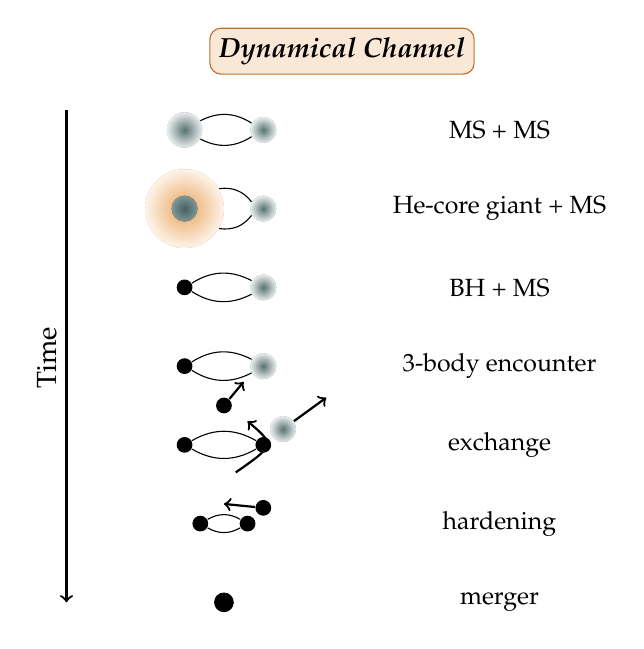
\begin{tikzpicture}

    \node at (2., 7) [title]{\itshape Dynamical Channel};
    
% Time arrow
    \draw[thick,->] (-1.5,6.25) -- (-1.5,0) node[midway,left,rotate=90, yshift=0.25cm,xshift=0.5cm] {Time};

    % Stage 1: MS + MS
    \node (ms1) at (0,6) [circle, fill=darkslategray!60, minimum size=0.45cm,, inner sep=0,shading=radial,inner color=darkslategray!80, outer color=darkslategray!10] {};
    \node (ms2) at (1,6) [circle, fill=darkslategray!60, minimum size=0.25cm,shading=radial,inner color=darkslategray!80, outer color=darkslategray!10] {};
    \draw (ms1) to[bend left=30] (ms2);
    \draw (ms2) to[bend left=30] (ms1);
    \node at (4,6) [align=center] {\small MS + MS};

    % Stage 2: He-core GIANT + MS
    \node (giant) at (0,5) [circle, fill=myorange, minimum size=1cm,shading=radial,inner color=myorange!80, outer color=myorange!10] {};
    \node (ms3) at (1,5) [circle, fill=darkslategray!60, minimum size=0.25cm,shading=radial,inner color=darkslategray!80, outer color=darkslategray!10] {};
    \draw (giant) to[bend left=30] (ms3);
    \draw (ms3) to[bend left=30] (giant);
    \node (ms4) at (0,5) [circle, fill=darkslategray!80, minimum size=0.25cm, ,shading=radial,inner color=darkslategray!90, outer color=darkslategray!60] {};
    \node at (4,5) [align=center]{\small{He-core giant + MS}};

    % Stage 3: BH + MS
    \node (bh1) at (0,4) [circle, fill=black, minimum size=0.2cm, inner sep=0] {};
    \node (ms4) at (1,4) [circle, fill=darkslategray!60, minimum size=0.25cm,shading=radial,inner color=darkslategray!80, outer color=darkslategray!10] {};
    \draw (bh1) to[bend left=30] (ms4);
    \draw (ms4) to[bend left=30] (bh1);
    \node at (4,4) [align=center]{\small BH + MS};

    % Stage 4: 3-BODY ENCOUNTER
    \node (bh2) at (0,3) [circle, fill=black, minimum size=0.2cm, inner sep=0] {};
    \node (ms5) at (1,3) [circle, fill=darkslategray!60, minimum size=0.25cm,shading=radial,inner color=darkslategray!80, outer color=darkslategray!10] {};
    \node (bh3) at (0.5,2.5) [circle, fill=black, minimum size=0.2cm, inner sep=0] {};
    \draw[->, thick] (bh3) -- (0.75,2.8);
    \draw (bh2) to[bend left=30] (ms5);
    \draw (ms5) to[bend left=30] (bh2);
    \node at (4,3) [align=center]{\small{3-body encounter}};

    % Stage 5: EXCHANGE
    \node (bh5) at (0,2) [circle, fill=black, minimum size=0.2cm, inner sep=0] {};
    \node (bh6) at (1,2) [circle, fill=black, minimum size=0.2cm, inner sep=0] {};
    \draw (bh5) to[bend left=30] (bh6);
    \draw (bh6) to[bend left=30] (bh5);
    \node (belowbh6) [below of=bh6] {};
    \node (abovebh6) [above of=bh6] {};
    \node (ms6) at (1.25,2.2) [circle, fill=darkslategray!60, minimum size=0.25cm,shading=radial,inner color=darkslategray!80, outer color=darkslategray!10] {};
    % Flyby arrow (curves around black hole)
    \draw[->, thick] (0.65,1.65) .. controls (1.15,2.) and (1.15,2.) .. (0.8,2.3);
    \draw[->, thick] (ms6) -- (1.8,2.6);
    \node at (4,2) [align=center]{\small exchange};

    % Stage 6: HARDENING
    \node (bh7) at (0.2,1) [circle, fill=black, minimum size=0.2cm, inner sep=0] {};
    \node (bh8) at (0.8,1) [circle, fill=black, minimum size=0.2cm, inner sep=0] {};
    \draw (bh7) to[bend left=30] (bh8);
    \draw (bh8) to[bend left=30] (bh7);
    \node (bh9) at (1,1.2) [circle, fill=black, minimum size=0.2cm, inner sep=0] {};
    \draw[->, thick] (bh9) -- (0.5,1.25);
    \node at (4,1) [align=center] {\small hardening};

    % Stage 7: MERGER
    \node (bh9) at (0.5,0) [circle, fill=black, minimum size=0.25cm, inner sep=0] {};
    \node at (4,0) [align=center] {\small merger};

\end{tikzpicture}
\end{document}
